\documentclass[letterpaper]{article}
\usepackage[margin=0mm]{geometry}
\usepackage[T1]{fontenc}
\usepackage{lmodern,tikz,amssymb}
\pdfmapfile{+lm.map}
\pdfmapfile{+symbols.map}
\usetikzlibrary{arrows.meta,calc}
\pagestyle{empty}
\setlength{\parindent}{0pt}
\begin{document}
\null\begin{tikzpicture}[remember picture,overlay,shift={(current page.north west)},x=1mm,y=-1mm,line cap=round,line join=round]
\node[anchor=north west,inner sep=0pt,text width=182mm,align=left,font=\fontsize{10.5}{13.125}\selectfont] at (16,11) {Week 39 / Road detours / Grades 2--3};
\draw[gray!55] (16,19)--(200,19);
\node[anchor=north west,inner sep=0pt,text width=180mm,align=left,font=\fontsize{11}{13.75}\selectfont] at (16,25) {Move a pawn on the roads. Keep each journey as ordered step tiles; an adult may record. Remove only two adjacent steps along the same road in opposite directions. Replay the other steps in order. The map, start, and finish stay fixed.};
\node[anchor=east,inner sep=1pt,font=\fontsize{9}{10.799999999999999}\selectfont] at (21,73) {input};
\draw[gray!45,line width=.3pt] (25,60) rectangle ++(31,26);
\draw[gray!40,line width=1mm] (30,77)--(40,77);
\draw[gray!40,line width=1mm] (40,77)--(40,67);
\draw[gray!40,line width=1mm] (40,77)--(50,77);
\draw[-{Stealth[length=2.3mm]},line width=1pt] (30,77)--(40,77);
\fill[red!65!black] (30,77) circle (1.2);
\node[anchor=center,inner sep=1pt,font=\fontsize{7}{8.4}\selectfont] at (30,73) {A};
\fill[blue!70!black] (40,77) circle (1.2);
\node[anchor=center,inner sep=1pt,font=\fontsize{7}{8.4}\selectfont] at (40,73) {B};
\fill[yellow!80!black] (40,67) circle (1.2);
\node[anchor=center,inner sep=1pt,font=\fontsize{7}{8.4}\selectfont] at (40,63) {C};
\fill[green!55!black] (50,77) circle (1.2);
\node[anchor=center,inner sep=1pt,font=\fontsize{7}{8.4}\selectfont] at (50,73) {D};
\draw[gray!45,line width=.3pt] (63,60) rectangle ++(31,26);
\draw[gray!40,line width=1mm] (68,77)--(78,77);
\draw[gray!40,line width=1mm] (78,77)--(78,67);
\draw[gray!40,line width=1mm] (78,77)--(88,77);
\draw[-{Stealth[length=2.3mm]},line width=1pt] (78,77)--(78,67);
\fill[red!65!black] (68,77) circle (1.2);
\node[anchor=center,inner sep=1pt,font=\fontsize{7}{8.4}\selectfont] at (68,73) {A};
\fill[blue!70!black] (78,77) circle (1.2);
\node[anchor=center,inner sep=1pt,font=\fontsize{7}{8.4}\selectfont] at (78,73) {B};
\fill[yellow!80!black] (78,67) circle (1.2);
\node[anchor=center,inner sep=1pt,font=\fontsize{7}{8.4}\selectfont] at (78,63) {C};
\fill[green!55!black] (88,77) circle (1.2);
\node[anchor=center,inner sep=1pt,font=\fontsize{7}{8.4}\selectfont] at (88,73) {D};
\draw[gray!45,line width=.3pt] (101,60) rectangle ++(31,26);
\draw[gray!40,line width=1mm] (106,77)--(116,77);
\draw[gray!40,line width=1mm] (116,77)--(116,67);
\draw[gray!40,line width=1mm] (116,77)--(126,77);
\draw[-{Stealth[length=2.3mm]},line width=1pt] (116,67)--(116,77);
\fill[red!65!black] (106,77) circle (1.2);
\node[anchor=center,inner sep=1pt,font=\fontsize{7}{8.4}\selectfont] at (106,73) {A};
\fill[blue!70!black] (116,77) circle (1.2);
\node[anchor=center,inner sep=1pt,font=\fontsize{7}{8.4}\selectfont] at (116,73) {B};
\fill[yellow!80!black] (116,67) circle (1.2);
\node[anchor=center,inner sep=1pt,font=\fontsize{7}{8.4}\selectfont] at (116,63) {C};
\fill[green!55!black] (126,77) circle (1.2);
\node[anchor=center,inner sep=1pt,font=\fontsize{7}{8.4}\selectfont] at (126,73) {D};
\draw[gray!45,line width=.3pt] (139,60) rectangle ++(31,26);
\draw[gray!40,line width=1mm] (144,77)--(154,77);
\draw[gray!40,line width=1mm] (154,77)--(154,67);
\draw[gray!40,line width=1mm] (154,77)--(164,77);
\draw[-{Stealth[length=2.3mm]},line width=1pt] (154,77)--(164,77);
\fill[red!65!black] (144,77) circle (1.2);
\node[anchor=center,inner sep=1pt,font=\fontsize{7}{8.4}\selectfont] at (144,73) {A};
\fill[blue!70!black] (154,77) circle (1.2);
\node[anchor=center,inner sep=1pt,font=\fontsize{7}{8.4}\selectfont] at (154,73) {B};
\fill[yellow!80!black] (154,67) circle (1.2);
\node[anchor=center,inner sep=1pt,font=\fontsize{7}{8.4}\selectfont] at (154,63) {C};
\fill[green!55!black] (164,77) circle (1.2);
\node[anchor=center,inner sep=1pt,font=\fontsize{7}{8.4}\selectfont] at (164,73) {D};
\node[anchor=center,inner sep=1pt,font=\fontsize{9}{10.799999999999999}\selectfont] at (193,73) {replay};
\node[anchor=east,inner sep=1pt,font=\fontsize{9}{10.799999999999999}\selectfont] at (21,107) {remove};
\draw[gray!45,line width=.3pt] (25,94) rectangle ++(31,26);
\draw[gray!40,line width=1mm] (30,111)--(40,111);
\draw[gray!40,line width=1mm] (40,111)--(40,101);
\draw[gray!40,line width=1mm] (40,111)--(50,111);
\draw[-{Stealth[length=2.3mm]},line width=1pt] (30,111)--(40,111);
\fill[red!65!black] (30,111) circle (1.2);
\node[anchor=center,inner sep=1pt,font=\fontsize{7}{8.4}\selectfont] at (30,107) {A};
\fill[blue!70!black] (40,111) circle (1.2);
\node[anchor=center,inner sep=1pt,font=\fontsize{7}{8.4}\selectfont] at (40,107) {B};
\fill[yellow!80!black] (40,101) circle (1.2);
\node[anchor=center,inner sep=1pt,font=\fontsize{7}{8.4}\selectfont] at (40,97) {C};
\fill[green!55!black] (50,111) circle (1.2);
\node[anchor=center,inner sep=1pt,font=\fontsize{7}{8.4}\selectfont] at (50,107) {D};
\draw[gray!45,line width=.3pt] (63,94) rectangle ++(31,26);
\draw[gray!40,line width=1mm] (68,111)--(78,111);
\draw[gray!40,line width=1mm] (78,111)--(78,101);
\draw[gray!40,line width=1mm] (78,111)--(88,111);
\draw[-{Stealth[length=2.3mm]},line width=1pt] (78,111)--(78,101);
\fill[red!65!black] (68,111) circle (1.2);
\node[anchor=center,inner sep=1pt,font=\fontsize{7}{8.4}\selectfont] at (68,107) {A};
\fill[blue!70!black] (78,111) circle (1.2);
\node[anchor=center,inner sep=1pt,font=\fontsize{7}{8.4}\selectfont] at (78,107) {B};
\fill[yellow!80!black] (78,101) circle (1.2);
\node[anchor=center,inner sep=1pt,font=\fontsize{7}{8.4}\selectfont] at (78,97) {C};
\fill[green!55!black] (88,111) circle (1.2);
\node[anchor=center,inner sep=1pt,font=\fontsize{7}{8.4}\selectfont] at (88,107) {D};
\draw[gray,line width=.7pt] (65,118)--(92,96);
\draw[gray!45,line width=.3pt] (101,94) rectangle ++(31,26);
\draw[gray!40,line width=1mm] (106,111)--(116,111);
\draw[gray!40,line width=1mm] (116,111)--(116,101);
\draw[gray!40,line width=1mm] (116,111)--(126,111);
\draw[-{Stealth[length=2.3mm]},line width=1pt] (116,101)--(116,111);
\fill[red!65!black] (106,111) circle (1.2);
\node[anchor=center,inner sep=1pt,font=\fontsize{7}{8.4}\selectfont] at (106,107) {A};
\fill[blue!70!black] (116,111) circle (1.2);
\node[anchor=center,inner sep=1pt,font=\fontsize{7}{8.4}\selectfont] at (116,107) {B};
\fill[yellow!80!black] (116,101) circle (1.2);
\node[anchor=center,inner sep=1pt,font=\fontsize{7}{8.4}\selectfont] at (116,97) {C};
\fill[green!55!black] (126,111) circle (1.2);
\node[anchor=center,inner sep=1pt,font=\fontsize{7}{8.4}\selectfont] at (126,107) {D};
\draw[gray,line width=.7pt] (103,118)--(130,96);
\draw[gray!45,line width=.3pt] (139,94) rectangle ++(31,26);
\draw[gray!40,line width=1mm] (144,111)--(154,111);
\draw[gray!40,line width=1mm] (154,111)--(154,101);
\draw[gray!40,line width=1mm] (154,111)--(164,111);
\draw[-{Stealth[length=2.3mm]},line width=1pt] (154,111)--(164,111);
\fill[red!65!black] (144,111) circle (1.2);
\node[anchor=center,inner sep=1pt,font=\fontsize{7}{8.4}\selectfont] at (144,107) {A};
\fill[blue!70!black] (154,111) circle (1.2);
\node[anchor=center,inner sep=1pt,font=\fontsize{7}{8.4}\selectfont] at (154,107) {B};
\fill[yellow!80!black] (154,101) circle (1.2);
\node[anchor=center,inner sep=1pt,font=\fontsize{7}{8.4}\selectfont] at (154,97) {C};
\fill[green!55!black] (164,111) circle (1.2);
\node[anchor=center,inner sep=1pt,font=\fontsize{7}{8.4}\selectfont] at (164,107) {D};
\node[anchor=center,inner sep=1pt,font=\fontsize{8}{9.6}\selectfont] at (193,107) {then replay};
\node[anchor=east,inner sep=1pt,font=\fontsize{9}{10.799999999999999}\selectfont] at (21,141) {output};
\draw[gray!45,line width=.3pt] (25,128) rectangle ++(31,26);
\draw[gray!40,line width=1mm] (30,145)--(40,145);
\draw[gray!40,line width=1mm] (40,145)--(40,135);
\draw[gray!40,line width=1mm] (40,145)--(50,145);
\draw[-{Stealth[length=2.3mm]},line width=1pt] (30,145)--(40,145);
\fill[red!65!black] (30,145) circle (1.2);
\node[anchor=center,inner sep=1pt,font=\fontsize{7}{8.4}\selectfont] at (30,141) {A};
\fill[blue!70!black] (40,145) circle (1.2);
\node[anchor=center,inner sep=1pt,font=\fontsize{7}{8.4}\selectfont] at (40,141) {B};
\fill[yellow!80!black] (40,135) circle (1.2);
\node[anchor=center,inner sep=1pt,font=\fontsize{7}{8.4}\selectfont] at (40,131) {C};
\fill[green!55!black] (50,145) circle (1.2);
\node[anchor=center,inner sep=1pt,font=\fontsize{7}{8.4}\selectfont] at (50,141) {D};
\draw[gray!45,line width=.3pt] (63,128) rectangle ++(31,26);
\draw[gray!40,line width=1mm] (68,145)--(78,145);
\draw[gray!40,line width=1mm] (78,145)--(78,135);
\draw[gray!40,line width=1mm] (78,145)--(88,145);
\draw[-{Stealth[length=2.3mm]},line width=1pt] (78,145)--(88,145);
\fill[red!65!black] (68,145) circle (1.2);
\node[anchor=center,inner sep=1pt,font=\fontsize{7}{8.4}\selectfont] at (68,141) {A};
\fill[blue!70!black] (78,145) circle (1.2);
\node[anchor=center,inner sep=1pt,font=\fontsize{7}{8.4}\selectfont] at (78,141) {B};
\fill[yellow!80!black] (78,135) circle (1.2);
\node[anchor=center,inner sep=1pt,font=\fontsize{7}{8.4}\selectfont] at (78,131) {C};
\fill[green!55!black] (88,145) circle (1.2);
\node[anchor=center,inner sep=1pt,font=\fontsize{7}{8.4}\selectfont] at (88,141) {D};
\node[anchor=north west,inner sep=0pt,text width=82mm,align=left,font=\fontsize{10}{12.5}\selectfont] at (111,134) {No steps left means the pawn stays at its start.};
\node[anchor=north west,inner sep=0pt,text width=180mm,align=left,font=\fontsize{12.5}{15.625}\selectfont] at (16,159) {\textbf{Problem 1:} Shorten each recorded trip until no move is possible. Make a different seven-step trip from C to F that finishes with the same route as the last one.};
\draw[line width=3mm,gray!25] (119,230)--(142,230);
\draw[line width=.7pt] (119,230)--(142,230);
\draw[line width=3mm,gray!25] (142,230)--(142,207);
\draw[line width=.7pt] (142,230)--(142,207);
\draw[line width=3mm,gray!25] (142,230)--(165,230);
\draw[line width=.7pt] (142,230)--(165,230);
\draw[line width=3mm,gray!25] (165,230)--(188,207);
\draw[line width=.7pt] (165,230)--(188,207);
\draw[line width=3mm,gray!25] (165,230)--(188,253);
\draw[line width=.7pt] (165,230)--(188,253);
\draw[fill=red!65!black!20,line width=.7pt] (119,230) circle (3.5);
\node[anchor=center,inner sep=1pt,font=\fontsize{12}{14.399999999999999}\selectfont] at (119,230) {A};
\draw[fill=blue!70!black!20,line width=.7pt] (142,230) circle (3.5);
\node[anchor=center,inner sep=1pt,font=\fontsize{12}{14.399999999999999}\selectfont] at (142,230) {B};
\draw[fill=yellow!80!black!20,line width=.7pt] (142,207) circle (3.5);
\node[anchor=center,inner sep=1pt,font=\fontsize{12}{14.399999999999999}\selectfont] at (142,207) {C};
\draw[fill=green!55!black!20,line width=.7pt] (165,230) circle (3.5);
\node[anchor=center,inner sep=1pt,font=\fontsize{12}{14.399999999999999}\selectfont] at (165,230) {D};
\draw[fill=orange!20,line width=.7pt] (188,207) circle (3.5);
\node[anchor=center,inner sep=1pt,font=\fontsize{12}{14.399999999999999}\selectfont] at (188,207) {E};
\draw[fill=violet!20,line width=.7pt] (188,253) circle (3.5);
\node[anchor=center,inner sep=1pt,font=\fontsize{12}{14.399999999999999}\selectfont] at (188,253) {F};
\node[anchor=north west,inner sep=0pt,text width=90mm,align=left,font=\fontsize{13}{16.25}\selectfont] at (19,207) {$A\to B\to A\to B\to D\to F\to D\to E$ $\longrightarrow$};
\node[anchor=north west,inner sep=0pt,text width=90mm,align=left,font=\fontsize{13}{16.25}\selectfont] at (19,228) {$A\to B\to D\to F\to D\to E$ $\longrightarrow$};
\node[anchor=north west,inner sep=0pt,text width=90mm,align=left,font=\fontsize{13}{16.25}\selectfont] at (19,249) {$C\to B\to C\to B\to D\to F$ $\longrightarrow$};
\node[anchor=north west,inner sep=0pt,text width=174mm,align=left,font=\fontsize{9}{11.25}\selectfont] at (16,266) {Bellingham Math Circle / Week 39 / F39-23-v2};
\node[anchor=center,inner sep=1pt,font=\fontsize{9}{10.799999999999999}\selectfont] at (198,268) {1};
\end{tikzpicture}
\newpage
\null\begin{tikzpicture}[remember picture,overlay,shift={(current page.north west)},x=1mm,y=-1mm,line cap=round,line join=round]
\node[anchor=north west,inner sep=0pt,text width=182mm,align=left,font=\fontsize{10.5}{13.125}\selectfont] at (16,11) {Week 39 / Road detours / Grades 2--3};
\draw[gray!55] (16,19)--(200,19);
\node[anchor=north west,inner sep=0pt,text width=180mm,align=left,font=\fontsize{12.5}{15.625}\selectfont] at (16,27) {\textbf{Problem 2:} Make three different 12-step trips from A back to A, each using every road. Can any trip home on this map survive after every immediate reversal is removed?};
\draw[line width=3mm,gray!25] (30,121)--(79,121);
\draw[line width=.7pt] (30,121)--(79,121);
\draw[line width=3mm,gray!25] (79,121)--(79,72);
\draw[line width=.7pt] (79,121)--(79,72);
\draw[line width=3mm,gray!25] (79,121)--(128,121);
\draw[line width=.7pt] (79,121)--(128,121);
\draw[line width=3mm,gray!25] (128,121)--(177,72);
\draw[line width=.7pt] (128,121)--(177,72);
\draw[line width=3mm,gray!25] (128,121)--(177,170);
\draw[line width=.7pt] (128,121)--(177,170);
\draw[fill=red!65!black!20,line width=.7pt] (30,121) circle (3.5);
\node[anchor=center,inner sep=1pt,font=\fontsize{12}{14.399999999999999}\selectfont] at (30,121) {A};
\draw[fill=blue!70!black!20,line width=.7pt] (79,121) circle (3.5);
\node[anchor=center,inner sep=1pt,font=\fontsize{12}{14.399999999999999}\selectfont] at (79,121) {B};
\draw[fill=yellow!80!black!20,line width=.7pt] (79,72) circle (3.5);
\node[anchor=center,inner sep=1pt,font=\fontsize{12}{14.399999999999999}\selectfont] at (79,72) {C};
\draw[fill=green!55!black!20,line width=.7pt] (128,121) circle (3.5);
\node[anchor=center,inner sep=1pt,font=\fontsize{12}{14.399999999999999}\selectfont] at (128,121) {D};
\draw[fill=orange!20,line width=.7pt] (177,72) circle (3.5);
\node[anchor=center,inner sep=1pt,font=\fontsize{12}{14.399999999999999}\selectfont] at (177,72) {E};
\draw[fill=violet!20,line width=.7pt] (177,170) circle (3.5);
\node[anchor=center,inner sep=1pt,font=\fontsize{12}{14.399999999999999}\selectfont] at (177,170) {F};
\draw[gray!45,line width=.3pt] (16,184) rectangle ++(180,71);
\node[anchor=north west,inner sep=0pt,text width=174mm,align=left,font=\fontsize{9}{11.25}\selectfont] at (16,266) {Bellingham Math Circle / Week 39 / F39-23-v2};
\node[anchor=center,inner sep=1pt,font=\fontsize{9}{10.799999999999999}\selectfont] at (198,268) {2};
\end{tikzpicture}
\newpage
\null\begin{tikzpicture}[remember picture,overlay,shift={(current page.north west)},x=1mm,y=-1mm,line cap=round,line join=round]
\node[anchor=north west,inner sep=0pt,text width=182mm,align=left,font=\fontsize{10.5}{13.125}\selectfont] at (16,11) {Week 39 / Road detours / Grades 2--3};
\draw[gray!55] (16,19)--(200,19);
\node[anchor=north west,inner sep=0pt,text width=180mm,align=left,font=\fontsize{12.5}{15.625}\selectfont] at (16,27) {\textbf{Problem 3:} Make every different trip from A back to A that can remain after shortening an eight-step ring trip. Find the fewest road steps in a surviving trip home.};
\draw[line width=3mm,gray!25] (55,119)--(103,71);
\draw[line width=.7pt] (55,119)--(103,71);
\draw[line width=3mm,gray!25] (103,71)--(151,119);
\draw[line width=.7pt] (103,71)--(151,119);
\draw[line width=3mm,gray!25] (151,119)--(103,167);
\draw[line width=.7pt] (151,119)--(103,167);
\draw[line width=3mm,gray!25] (103,167)--(55,119);
\draw[line width=.7pt] (103,167)--(55,119);
\draw[fill=red!65!black!20,line width=.7pt] (55,119) circle (3.5);
\node[anchor=center,inner sep=1pt,font=\fontsize{12}{14.399999999999999}\selectfont] at (55,119) {A};
\draw[fill=blue!70!black!20,line width=.7pt] (103,71) circle (3.5);
\node[anchor=center,inner sep=1pt,font=\fontsize{12}{14.399999999999999}\selectfont] at (103,71) {B};
\draw[fill=yellow!80!black!20,line width=.7pt] (151,119) circle (3.5);
\node[anchor=center,inner sep=1pt,font=\fontsize{12}{14.399999999999999}\selectfont] at (151,119) {C};
\draw[fill=green!55!black!20,line width=.7pt] (103,167) circle (3.5);
\node[anchor=center,inner sep=1pt,font=\fontsize{12}{14.399999999999999}\selectfont] at (103,167) {D};
\node[anchor=north west,inner sep=0pt,text width=180mm,align=left,font=\fontsize{12.5}{15.625}\selectfont] at (16,189) {\textbf{Problem 4:} Remove different first detours from the recorded trip below. Can two removal orders end differently?};
\node[anchor=north west,inner sep=0pt,text width=175mm,align=left,font=\fontsize{13}{16.25}\selectfont] at (19,221) {$A\to B\to A\to B\to C\to B\to A\to D\to C\to D\to A$\hfill $\longrightarrow$ \rule{48mm}{.3pt}};
\draw[gray!45,line width=.3pt] (16,243) rectangle ++(180,13);
\node[anchor=north west,inner sep=0pt,text width=174mm,align=left,font=\fontsize{9}{11.25}\selectfont] at (16,266) {Bellingham Math Circle / Week 39 / F39-23-v2};
\node[anchor=center,inner sep=1pt,font=\fontsize{9}{10.799999999999999}\selectfont] at (198,268) {3};
\end{tikzpicture}
\newpage
\null\begin{tikzpicture}[remember picture,overlay,shift={(current page.north west)},x=1mm,y=-1mm,line cap=round,line join=round]
\node[anchor=north west,inner sep=0pt,text width=182mm,align=left,font=\fontsize{10.5}{13.125}\selectfont] at (16,11) {Week 39 / Road detours / Grades 2--3};
\draw[gray!55] (16,19)--(200,19);
\node[anchor=north west,inner sep=0pt,text width=180mm,align=left,font=\fontsize{12.5}{15.625}\selectfont] at (16,27) {\textbf{Problem 5:} From H, go around the left ring through A, then the right ring through C. Trade only the order of the two full ring trips. Do the two journeys become the same after removing every immediate reversal?};
\draw[line width=3mm,gray!25] (107,128)--(25,87);
\draw[line width=.7pt] (107,128)--(25,87);
\draw[line width=3mm,gray!25] (25,87)--(25,169);
\draw[line width=.7pt] (25,87)--(25,169);
\draw[line width=3mm,gray!25] (25,169)--(107,128);
\draw[line width=.7pt] (25,169)--(107,128);
\draw[line width=3mm,gray!25] (107,128)--(189,87);
\draw[line width=.7pt] (107,128)--(189,87);
\draw[line width=3mm,gray!25] (189,87)--(189,169);
\draw[line width=.7pt] (189,87)--(189,169);
\draw[line width=3mm,gray!25] (189,169)--(107,128);
\draw[line width=.7pt] (189,169)--(107,128);
\draw[fill=black!20,line width=.7pt] (107,128) circle (3.5);
\node[anchor=center,inner sep=1pt,font=\fontsize{12}{14.399999999999999}\selectfont] at (107,128) {H};
\draw[fill=red!65!black!20,line width=.7pt] (25,87) circle (3.5);
\node[anchor=center,inner sep=1pt,font=\fontsize{12}{14.399999999999999}\selectfont] at (25,87) {A};
\draw[fill=blue!70!black!20,line width=.7pt] (25,169) circle (3.5);
\node[anchor=center,inner sep=1pt,font=\fontsize{12}{14.399999999999999}\selectfont] at (25,169) {B};
\draw[fill=yellow!80!black!20,line width=.7pt] (189,87) circle (3.5);
\node[anchor=center,inner sep=1pt,font=\fontsize{12}{14.399999999999999}\selectfont] at (189,87) {C};
\draw[fill=green!55!black!20,line width=.7pt] (189,169) circle (3.5);
\node[anchor=center,inner sep=1pt,font=\fontsize{12}{14.399999999999999}\selectfont] at (189,169) {D};
\node[anchor=north west,inner sep=0pt,text width=180mm,align=left,font=\fontsize{12.5}{15.625}\selectfont] at (16,197) {\textbf{Problem 6:} Make two trips from H back to H, each using both rings and at least 12 road steps. One must shorten to staying at H; the other must lose no steps.};
\draw[gray!45,line width=.3pt] (16,235) rectangle ++(180,21);
\node[anchor=north west,inner sep=0pt,text width=174mm,align=left,font=\fontsize{9}{11.25}\selectfont] at (16,266) {Bellingham Math Circle / Week 39 / F39-23-v2};
\node[anchor=center,inner sep=1pt,font=\fontsize{9}{10.799999999999999}\selectfont] at (198,268) {4};
\end{tikzpicture}
\end{document}
